\section{Einleitung} % (fold)
\label{sec:einleitung}

% section einleitung (end)



\section{Motivation} % (fold)
\label{sub:motivation}

	Larry Page, CEO und Mitgründer von Google, sagt:
	\begin{quote}
		\textit{"`As a product manager you should know that speed is the number one feature."'}\autocite{}
	\end{quote}
	Niemand mag es zu warten, auch nicht auf eine Website. Die Studie "`The Psychology of Web Performance"' kam bereits im Jahr 2008 schon auf folgende Ergebnisse:

	\begin{quote}\itshape
		"`Slow web pages lower perceived credibility and quality. Keep your page load times below tolerable attention thresholds, and users will experience less frustration, lower blood pressure, deeper flow states, higher conversion rates, and lower bailout rates. Faster websites are actually perceived to be more interesting and attractive."' \autocite{webOpti08}
	\end{quote}

	Tatsächlich ist für Google Geschwindigkeit alles. Das haupt Vermarktungsargument für den Chrome Browser war damals: er sei schneller als die Konkurenz.	Deshalb hat Google im Jahr 2010 angekündigt, dass Geschwindigkeit in die Berechnung des \texttt{Page Rankings} mit einfließt.

	\begin{quote}\itshape
		"`Faster sites create happy users and we've seen in our internal studies that when a site responds slowly, visitors spend less time there. [...] Recent data shows that improving site speed also reduces operating costs. Like us, our users place a lot of value in speed — that's why we've decided to take site speed into account in our search rankings"'\autocite{google10}
	\end{quote}

	Aktuell (2015) geht Google sogar noch einen Schritt weiter und informiert tausende Webmaster per E-Mail über die schlechte Usability ihrer Websites für mobile Besucher und warnt ausdrücklich vor dementsprechend "`angepassten Rankings"'.\autocite{t3n15}
	Im Hinblick auf die Zukunft wird der Marktanteil an mobilen Internetnutzern noch weiter wachsen und die Optimierung der Ladezeiten gewinnt dadurch noch mehr an bedeutung. Zwischen 2011 und 2014 stieg die Anzahl der Smartphone nutzer von 18\% auf 50\% an. Dies ist ein Wachstum von 32\% innerhalb von nur 3 Jahren.\autocite{tns14}\\

	\begin{figure}[htbp]
		\begin{center}
			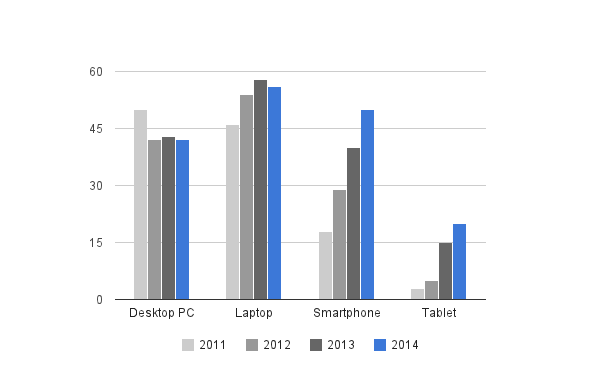
\includegraphics[width=0.75\textwidth]{smartphoneUsage.png}
		\end{center}
		\caption{Gerätenutzung in der Gesamtbevölkerung (2011 – 2014)\autocite{tns14}}
		\label{fig:geraetenutzung}
	\end{figure}

	Die Antwort auf diesen Trend läutete eine Ära ein, die wir heute unter dem Namen \texttt{Responsive Webdesign} kennen. "`Responsive"' muss aber sehr viel mehr bedeuten, als nur eine angepasste Darstellung für eine bestimmte Art von Gerät. "`Two out of three mobile shoppers expect pages to load in 4 seconds or less."' \autocite{radware13}. Der Anwender erwartet also auf dem Smartphone änliche oder gleiche Ladezeiten wie er auch von der Nutzung eines Desktop-Pc's gewohnt ist.

	Der Inhalt einer Seite muss darum so aufbereitet werden, dass dieser auch auf Geräten mit langsamer Internetverbindung, hoher Latenz und einem begrenzten Datentarif, in einer für den Anwender annehmbaren Geschwindigkeit, angezeigt werden kann.\\

% subsection motivation (end)


\subsection{Zielsetzung} % (fold)
\label{sub:zielsetzung}
	Um gängige Methoden und Techniken der Performance Optimierung anzuwenden wird das Projekt anhand der Webseite \url{http://andreaslorer.de} durchgeführt.

% subsection zielsetzung (end)



\section{Eigene Leistung} % (fold)
\label{sub:eigene_leistung}

% subsection eigene_leistung (end)



\section{Ist-Zustand} % (fold)
\label{sec:Ist-Zustand}

% section  (end)
